% License
%    This file is part of GitHub "EEE-DA" (https://github.com/julemai/EEE-DA) 
%    providing data and scripts to reproduce all figures of the publication:
%
%       J. Mai, R. Arsenault, B.A. Tolson, M. Latraverse, and K. Demeester (2020).
%       Application of Parameter Screening To Derive Optimal Initial State 
%       Adjustments for Streamflow Forecasting.
%       Water Resources Research, ??, ???-???.
%       https://doi.org/10.1002/???.
%
%    The EEE-DA codes are under MIT license.
%
%    Permission is hereby granted, free of charge, to any person obtaining a copy
%    of this software and associated documentation files (the "Software"), to deal
%    in the Software without restriction, including without limitation the rights
%    to use, copy, modify, merge, publish, distribute, sublicense, and/or sell
%    copies of the Software, and to permit persons to whom the Software is
%    furnished to do so, subject to the following conditions:
%
%    The above copyright notice and this permission notice shall be included in all
%    copies or substantial portions of the Software.
%
%    THE SOFTWARE IS PROVIDED "AS IS", WITHOUT WARRANTY OF ANY KIND, EXPRESS OR
%    IMPLIED, INCLUDING BUT NOT LIMITED TO THE WARRANTIES OF MERCHANTABILITY,
%    FITNESS FOR A PARTICULAR PURPOSE AND NONINFRINGEMENT. IN NO EVENT SHALL THE
%    AUTHORS OR COPYRIGHT HOLDERS BE LIABLE FOR ANY CLAIM, DAMAGES OR OTHER
%    LIABILITY, WHETHER IN AN ACTION OF CONTRACT, TORT OR OTHERWISE, ARISING FROM,
%    OUT OF OR IN CONNECTION WITH THE SOFTWARE OR THE USE OR OTHER DEALINGS IN THE
%    SOFTWARE.


\documentclass{article}

%\usepackage[math,lf,footnotefigures]{MyriadPro}
\renewcommand\familydefault{\sfdefault} 
%\usepackage[T1]{fontenc}

\usepackage{tikz}
\usetikzlibrary{arrows}
\usetikzlibrary{arrows.meta}
\usetikzlibrary{positioning}

\usepackage{xcolor}
\definecolor{ufzgray1}{RGB}{81,81,81}
\definecolor{ufzgray2}{RGB}{156,156,156}
\definecolor{ufzgray3}{RGB}{185,185,185}
\definecolor{ufzgray4}{RGB}{230,230,230}

\begin{document}
	
\pagestyle{empty}

\hspace*{-3cm}
	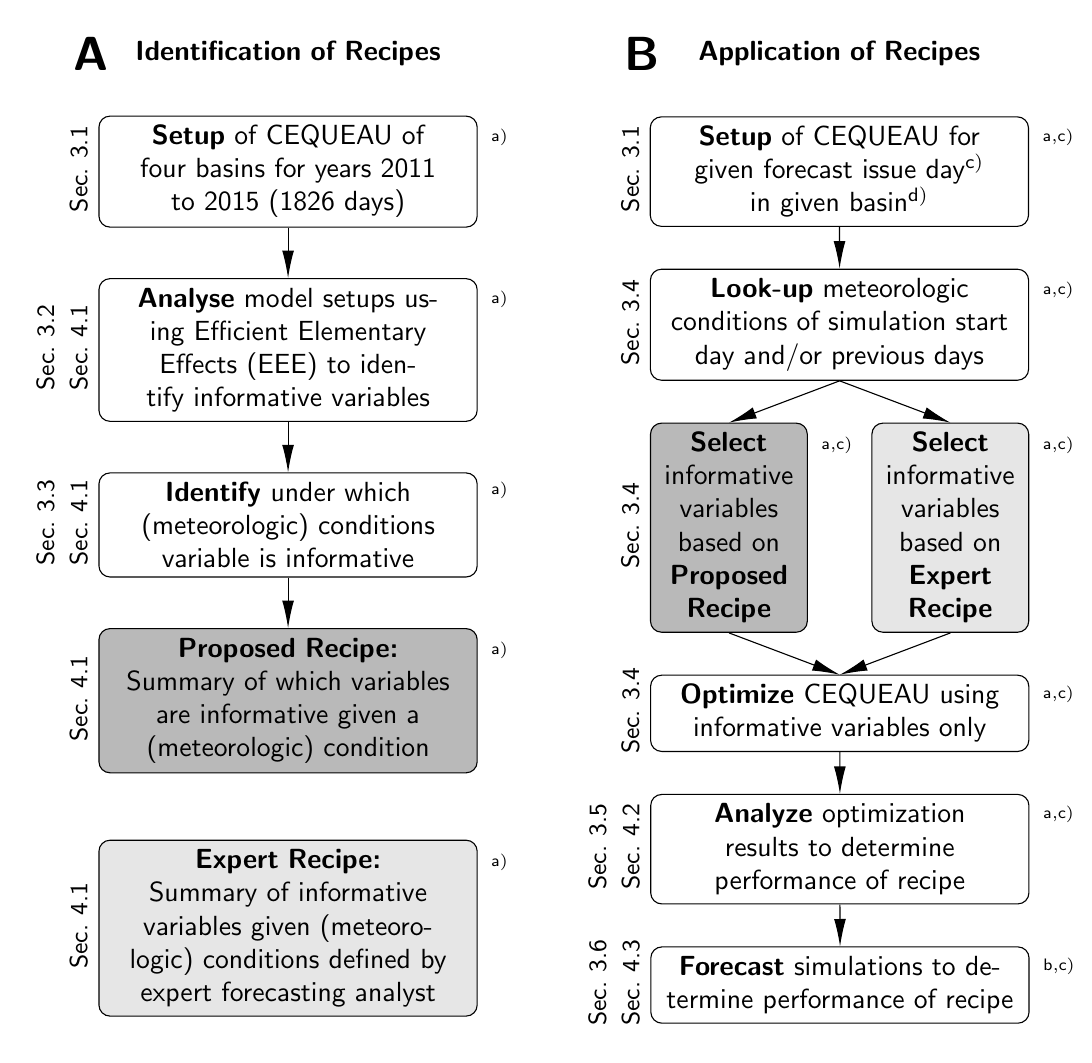
\begin{tikzpicture}[scale=2.5]
		\tikzstyle{block} = [rectangle, draw, fill=white!20, 
		text width=13em, text centered, rounded corners, minimum height=1em]
		\tikzstyle{noblock} = [rectangle, fill=white!20, 
		text width=14em, rounded corners, minimum height=1em]
		\tikzstyle{abcblock} = [rectangle, fill=white!20, 
		text width=1em, rounded corners, minimum height=1em]
		\tikzstyle{line} = [draw, -latex']
		\tikzstyle{line} = [draw,latex'-latex'new]
		
		% caption
		\node [noblock,align=center] (A) {\textbf{Identification of Recipes}};
		\node [noblock,align=center,right of=A,xshift=6cm] (B) {\textbf{Application of Recipes}};
		
		% ABC
		\node [abcblock,align=center,left of=A,xshift=-1.55cm] {{\LARGE \textbf{A}}};
		\node [abcblock,align=center,left of=B,xshift=-1.55cm] {{\LARGE \textbf{B}}};
		
		% Identification of Recipes
		\node [block, below of=A, node distance=1.5cm] (a1) {\textbf{Setup} of CEQUEAU of four basins for years 2011 to 2015 (1826 days)};
		\node [noblock,rotate=90,align=center,left=0.25cm of a1.west,text width=0.4em,xshift=-0.25cm] (a1sec) {\small Sec.~3.1};
		\node [noblock,rotate=0,align=left,right=0.05cm of a1.east,text width=0.4em,xshift=0.0cm,yshift=0.4cm] (a1note) {\small $^\mathsf{a)}$};
		
		\node [block, below=0.64cm of a1.south, node distance=2.5cm] (a2) {\textbf{Analyse} model setups using Efficient Elementary Effects (EEE) to identify informative variables};
		\node [noblock,rotate=90,align=center,left=0.46cm of a2.west,text width=0.4em,xshift=-0.25cm] (a2sec) {\small Sec.~3.2\\Sec.~4.1};
		\node [noblock,rotate=0,align=left,right=0.05cm of a2.east,text width=0.4em,xshift=0.0cm,yshift=0.6cm] (a2note) {\small $^\mathsf{a)}$};
		
		\node [block, below=0.64cm of a2.south, node distance=2.5cm] (a3) {\textbf{Identify} under which (meteorologic) conditions variable is informative};
		\node [noblock,rotate=90,align=center,left=0.46cm of a3.west,text width=0.4em,xshift=-0.25cm] (a2sec) {\small Sec.~3.3\\Sec.~4.1};
		\node [noblock,rotate=0,align=left,right=0.05cm of a3.east,text width=0.4em,xshift=0.0cm,yshift=0.4cm] (a3note) {\small $^\mathsf{a)}$};
		
		\node [block, below=0.64cm of a3.south, node distance=2.5cm, fill=ufzgray3] (a4) {\textbf{Proposed Recipe:}\\ Summary of which variables are informative given a (meteorologic) condition};
		\node [noblock,rotate=90,align=center,left=0.25cm of a4.west,text width=0.4em,xshift=-0.25cm] (a2sec) {\small Sec.~4.1};
		\node [noblock,rotate=0,align=left,right=0.05cm of a4.east,text width=0.4em,xshift=0.0cm,yshift=0.6cm] (a4note) {\small $^\mathsf{a)}$};
		
		\node [block, below=0.84cm of a4.south, node distance=2.5cm, fill=ufzgray4] (a5) {\textbf{Expert Recipe:}\\ Summary of informative variables given (meteorologic) conditions defined by expert forecasting analyst};
		\node [noblock,rotate=90,align=center,left=0.25cm of a5.west,text width=0.4em,xshift=-0.25cm] (a2sec) {\small Sec.~4.1};
		\node [noblock,rotate=0,align=left,right=0.05cm of a5.east,text width=0.4em,xshift=0.0cm,yshift=0.8cm] (a5note) {\small $^\mathsf{a)}$};
		
		\node [block, below of=B, node distance=1.5cm] (b1) {\textbf{Setup} of CEQUEAU for\\ given forecast issue day$^\mathsf{c)}$ \\ in given basin$^\mathsf{d)}$};
		\node [noblock,rotate=90,align=center,left=0.25cm of b1.west,text width=0.4em,xshift=-0.25cm] (b2sec) {\small Sec.~3.1};
		\node [noblock,rotate=0,align=left,right=0.05cm of b1.east,text width=0.4em,xshift=0.0cm,yshift=0.4cm] (b1note) {\small $^\mathsf{a,c)}$};
				
		\node [block, below=0.53cm of b1.south, node distance=2.5cm] (b2) {\textbf{Look-up} meteorologic conditions of simulation start day and/or previous days};
		\node [noblock,rotate=90,align=center,left=0.25cm of b2.west,text width=0.4em,xshift=-0.25cm] (b2sec) {\small Sec.~3.4};
		\node [noblock,rotate=0,align=left,right=0.05cm of b2.east,text width=0.4em,xshift=0.0cm,yshift=0.4cm] (b2note) {\small $^\mathsf{a,c)}$};
		
		\node [block, below=0.53cm of b2.south, node distance=2.5cm, text width=5.0em, xshift=-4.0em, fill=ufzgray3] (b3a) {\textbf{Select} informative variables based on \textbf{Proposed Recipe}};
		\node [block, below=0.53cm of b2.south, node distance=2.5cm, text width=5.0em, xshift=4.0em, fill=ufzgray4] (b3b) {\textbf{Select} informative variables based on \textbf{Expert Recipe}};
		\node [noblock,rotate=90,align=center,left=0.25cm of b3a.west,text width=0.4em,xshift=-0.25cm] (b3sec) {\small Sec.~3.4};
		\node [noblock,rotate=0,align=left,right=0.05cm of b3a.east,text width=0.4em,xshift=0.0cm,yshift=1.0cm] (b3anote) {\small $^\mathsf{a,c)}$};
		\node [noblock,rotate=0,align=left,right=0.05cm of b3b.east,text width=0.4em,xshift=0.0cm,yshift=1.0cm] (b3bnote) {\small $^\mathsf{a,c)}$};
		
		\node [block, below=0.53cm of b3a.south, node distance=2.5cm, xshift=4.0em] (b4) {\textbf{Optimize} CEQUEAU using informative variables only};
		\node [noblock,rotate=90,align=center,left=0.25cm of b4.west,text width=0.4em,xshift=-0.25cm] (b4sec) {\small Sec.~3.4};
		\node [noblock,rotate=0,align=left,right=0.05cm of b4.east,text width=0.4em,xshift=0.0cm,yshift=0.2cm] (b4note) {\small $^\mathsf{a,c)}$};
		
		\node [block, below=0.53cm of b4.south, node distance=2.5cm] (b5) {\textbf{Analyze} optimization results to determine performance of recipe};
		\node [noblock,rotate=90,align=center,left=0.46cm of b5.west,text width=0.4em,xshift=-0.25cm] (b5sec) {\small Sec.~3.5\\Sec.~4.2};
		\node [noblock,rotate=0,align=left,right=0.05cm of b5.east,text width=0.4em,xshift=0.0cm,yshift=0.4cm] (b5note) {\small $^\mathsf{a,c)}$};
		
		\node [block, below=0.53cm of b5.south, node distance=2.5cm] (b6) {\textbf{Forecast} simulations to determine performance of recipe};
		\node [noblock,rotate=90,align=center,left=0.46cm of b6.west,text width=0.4em,xshift=-0.25cm] (b5sec) {\small Sec.~3.6\\Sec.~4.3};
		\node [noblock,rotate=0,align=left,right=0.05cm of b6.east,text width=0.4em,xshift=0.0cm,yshift=0.2cm] (b6note) {\small $^\mathsf{b,c)}$};
		
		% lines A-B (realistic setup)
		\draw [-{Latex[length=3.5mm, width=1.5mm]}] (a1.south) -- (a2.north);
		\draw [-{Latex[length=3.5mm, width=1.5mm]}] (a2.south) -- (a3.north);
		\draw [-{Latex[length=3.5mm, width=1.5mm]}] (a3.south) -- (a4.north);
		
		\draw [-{Latex[length=3.5mm, width=1.5mm]}] (b1.south) -- (b2.north);
		\draw [-{Latex[length=3.5mm, width=1.5mm]}] (b2.south) -- (b3a.north);
		\draw [-{Latex[length=3.5mm, width=1.5mm]}] (b2.south) -- (b3b.north);
		\draw [-{Latex[length=3.5mm, width=1.5mm]}] (b3a.south) -- (b4.north);
		\draw [-{Latex[length=3.5mm, width=1.5mm]}] (b3b.south) -- (b4.north);
		\draw [-{Latex[length=3.5mm, width=1.5mm]}] (b4.south) -- (b5.north);
		\draw [-{Latex[length=3.5mm, width=1.5mm]}] (b5.south) -- (b6.north);
		
	\end{tikzpicture}

\end{document}



